\documentclass[british]{article}
\usepackage[T1]{fontenc}
\usepackage[latin9]{inputenc}
\usepackage{geometry}
\geometry{verbose,tmargin=3.5cm,bmargin=3.5cm,lmargin=3cm,rmargin=3cm}
\usepackage{array}
%\usepackage{multirow}
\usepackage{amstext}
\usepackage{graphicx}
\usepackage{color}
\usepackage{caption}
%\usepackage{subfigure}

\newcommand{\tabincell}[2]{\begin{tabular}{@{}#1@{}}#2\end{tabular}}

\newcommand{\mytablefontsize}{7pt}
\newcommand{\mytablebaselineskip}{0.7}
\newcommand{\mytabcolsep}{3pt}

\newcommand{\medianInterval}[1]{}


\makeatletter

%%%%%%%%%%%%%%%%%%%%%%%%%%%%%% LyX specific LaTeX commands.
%% Because html converters don't know tabularnewline
\providecommand{\tabularnewline}{\\}

%%%%%%%%%%%%%%%%%%%%%%%%%%%%%% User specified LaTeX commands.

\title{Configuration Reports for the Solver PbO-CCSAT-Generic on the Instance Sset PTN in \emph{Sparkle} }
\author{ Automatically generated by \emph{Sparkle} (version: 1.0.0) }

\makeatother

\usepackage{babel}
\begin{document}
\maketitle %


\section{Introduction}
\label{sec:Introduction}

\emph{Sparkle} \cite{Hoos15} is a multi-agent problem-solving platform based on Programming by Optimisation (PbO) \cite{Hoos12}, and would provide a number of effective algorithm optimisation techniques (such as automated algorithm configuration, portfolio-based algorithm selection, etc) to accelerate the existing solvers.

This experimental report is automatically generated by \emph{Sparkle}. This report presents experimental results on the scenario of configuring the solver PbO-CCSAT-Generic on the instance set PTN.

\section{Information about the Instance Set}

The whole instance set is PTN, and there are 23 instances in the whole instance set. First of all, \emph{Sparkle} selected two subsets from the whole instance set as the training set and the testing set. The information about the training set and the testing set is presented as follows.

\begin{itemize}
\item Training set: 11 instances
\item Testing set: 12 instances
\end{itemize}

\section{Information about the Configuration Protocol}

The configurator used in \emph{Sparkle} is SMAC ({\em Sequential Model-based Algorithm Configuration}) \cite{HutEtAl11}, and the version of SMAC used in \emph{Sparkle} is 2.10.03.

During the configuration process, \emph{Sparkle} performs 25 independent SMAC runs for configuring the solver PbO-CCSAT-Generic on the instance set PTN; the configuration objective is RUNTIME; the whole configuration time budget is 300 seconds; the cutoff time for each run is 60 seconds.

Each independent run of SMAC would result in one optimised configuration. As a result, \emph{Sparkle} would obtain 25 optimised configurations. Each of these was then evaluated on the entire training set, with one solver run per instance and a cutoff time of 60 seconds, and the configuration with the lowest PAR10 value was selected as the result of the configuration process.

\section{Information about the Optimised Configuration}

After the configuration process mentioned above, \emph{Sparkle} obtained the optimised configuration. The details of the optimised configuration are described as below.

\vspace{5mm}

 -gamma\textunderscore hscore2 '351' -init\textunderscore solution '1' -p\textunderscore swt '0.20423712003341465' -perform\textunderscore aspiration '1' -perform\textunderscore clause\textunderscore weight '1' -perform\textunderscore double\textunderscore cc '0' -perform\textunderscore first\textunderscore div '0' -perform\textunderscore pac '1' -prob\textunderscore pac '0.005730374136488115' -q\textunderscore swt '0.6807207179674418' -sel\textunderscore clause\textunderscore div '1' -sel\textunderscore clause\textunderscore weight\textunderscore scheme '1' -sel\textunderscore var\textunderscore break\textunderscore tie\textunderscore greedy '4' -sel\textunderscore var\textunderscore div '2' -threshold\textunderscore swt '32'

\vspace{5mm}

%The PAR10 value of the optimised configuration on the entire training set is 8.500000.

\section{Comparison between Configured Version and Default Version on the Testing Instance Set}

After specifying the optimised configuration, \emph{Sparkle} would run the configured version of PbO-CCSAT-Generic and the default version of PbO-CCSAT-Generic on the testing instance set. During this phase, each version was performed one run per instance with a cutoff time of 60 seconds. The results are reported as follows.

\begin{itemize}
\item \textbf{PbO-CCSAT-Generic (configured)}, PAR10: 5.770833
\item \textbf{PbO-CCSAT-Generic (default)}, PAR10: 451.110000
\end{itemize}

The empirical comparison between the PbO-CCSAT-Generic (configured) and PbO-CCSAT-Generic (default) on the testing set of PTN is presented in Figure \ref{fig:configured_vs_default_test}.

\begin{figure}[htbp]
\noindent \begin{centering}
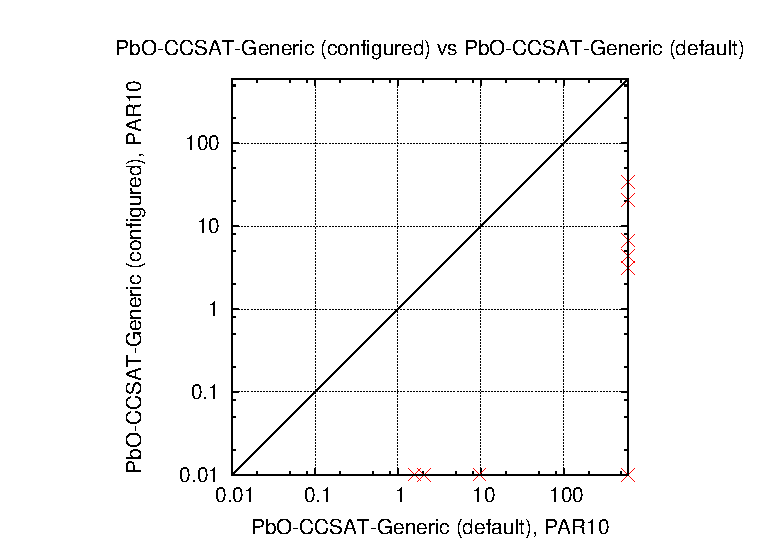
\includegraphics[width=0.6\textwidth]{data_PbO-CCSAT-Generic_configured_vs_default_on_PTN_test}
% \includegraphics[width=0.8\textwidth]{fittedModels}
\par\end{centering}

\caption{Empirical comparison between the PbO-CCSAT-Generic (configured) and PbO-CCSAT-Generic (default) on the testing set of PTN.}\label{fig:configured_vs_default_test}
\end{figure}


\section{Comparison between Configured Version and Default Version on the Training Instance Set}
In order to investigate the performance on the training instance set, \emph{Sparkle} would run the configured version of PbO-CCSAT-Generic and the default version of PbO-CCSAT-Generic on the training instance set. During this phase, each version was performed one run per instance with a cutoff time of 60 seconds. The results are reported as follows.

\begin{itemize}
\item \textbf{PbO-CCSAT-Generic (configured)}, PAR10: 8.500000
\item \textbf{PbO-CCSAT-Generic (default)}, PAR10: 287.646364
\end{itemize}

The empirical comparison between the PbO-CCSAT-Generic (configured) and PbO-CCSAT-Generic (default) on the training set of PTN is presented in Figure \ref{fig:configured_vs_default_train}.

\begin{figure}[htbp]
\noindent \begin{centering}
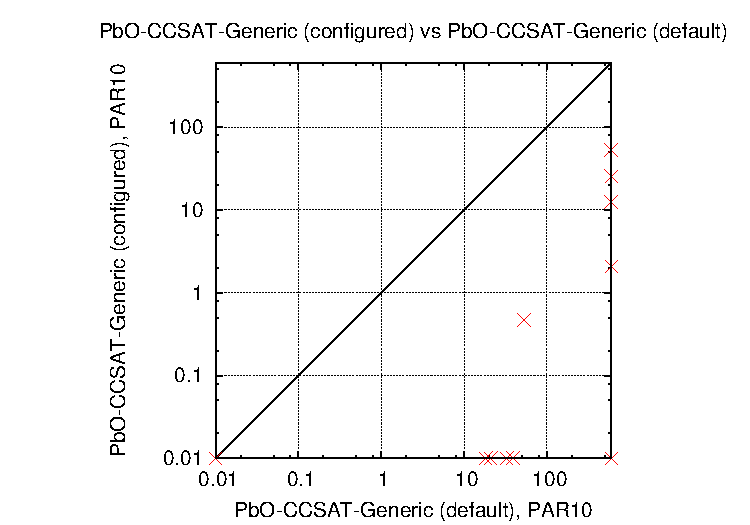
\includegraphics[width=0.6\textwidth]{data_PbO-CCSAT-Generic_configured_vs_default_on_PTN_train}
% \includegraphics[width=0.8\textwidth]{fittedModels}
\par\end{centering}

\caption{Empirical comparison between the PbO-CCSAT-Generic (configured) and PbO-CCSAT-Generic (default) on the training set of PTN.}\label{fig:configured_vs_default_train}
\end{figure}


\bibliographystyle{plain}
\bibliography{Sparkle_Report_for_Configuration}

\end{document}
